\chapter{Background}

This chapter will provide the theoretical background for this thesis. First, we will discuss the field of multi-robot systems, providing the reader with an understanding of how the field has evolved and how it may further evolve. Next, we examine RobotWeb \cite{Robotweb}, the research that this thesis seeks to build upon. Finally, we discuss various security issues present in the field to arrive at the research question for this thesis.

\section{Multi-Robot Systems} % QUESTION: Can I call this Distributed Robotics??
The study of multi-robot systems concerns itself with studying how to allow multiple robots to operate in the same environment \cite{MRS-Implicit-Explicit-Comms}. Multi-robot systems have several advantages over single-robot systems; they are more effective, efficient, flexible, and resilient \cite{MultiVsSingleRobotSystems}. These robots can behave competitively or collaboratively, coordinate statically or dynamically, communicate explicitly or implicitly, consist of homogeneous or heterogeneous robots, and make decisions centrally or decentrally \cite{MultiRobotCoordinationSurvey}. % QUESTION: Can I cite this paper at all / am I citing it too much?
% QUESTION: Is the evolve sentence all right or not?

\subsection{Competitive vs Collaborative Behavior}
Multiple robots which share a common goal are considered to be behaving collaboratively, whereas if each robot aimed to complete its own goal at the expense of all others, it would be said to be behaving competitively \cite{MultiRobotCoordinationSurvey}. Examples of collaboration range from teams of robots constructing a lunar habitat \cite{LunarHabitatConstructionExample} to exploring unknown environments \cite{MultiRobotExplorationExample}.

\subsection{Static vs Dynamic Coordination}
If a multi-robot system operates using a set of predetermined rules, then it can be said to be coordinating itself statically \cite{MultiRobotCoordinationSurvey}. A possible set of rules would be that each robot must maintain a certain distance between it and all others \cite{MultiRobotCoordinationSurvey}. Dynamically coordinated multi-robot systems would instead make decisions whilst performing the task and may communicate to do so \cite{MultiRobotCoordinationSurvey}.

\subsection{Explicit vs Implicit Communication}
Most multi-robot systems communicate explicitly by sending messages to each other via a hardware communication interface, for example, a wifi module \cite{MultiRobotCoordinationSurvey}. However, there is still a sizeable minority of approaches that send messages through their environment (implicit communication) and rely on others to sense these messages to receive them. An example of implicit communication is found in \cite{FootballRobots}, where the authors use it to allow a team of robots to play a game of football for the RoboCup Simulation League \cite{RoboCup}.

\subsection{Homogeneous vs Heterogeneous Robots}
Multi-robot systems can either contain robots with identical hardware, which are known as homogeneous systems, or individual robots may have different hardware, making them heterogeneous systems. Heterogeneous systems allow a greater degree of specialisation within a multi-robot system but also add additional decision-making complexity.

\subsection{Centralised vs Decentralised Decision Making}
A multi-robot system is said to have centralised decision-making if all robots communicate with a central agent, which may or may not be a robot itself, to receive instructions. Centralised schemes perform better with smaller groups of robots and in static environments, they also introduce a single point of failure in the central agent \cite{MultiRobotCoordinationSurvey}. Decentralised schemes, however, avoid vesting authority into a central agent and instead treat each agent as an equal part of the system, which allows them to avoid the problems associated with centralised schemes. However, decentralised schemes lose the guarantee that they will converge to an optimal solution, as decisions are made with incomplete information. % Should I add more citations here?
In addition to centralised and decentralised schemes, multi-robot systems may also be organised in a hierarchical manner, where some robots would be chosen as local leaders, but no global leader would exist.

\section{Robot Web}
This thesis seeks to build upon the work done in ``A Robot Web for Distributed Many-Device Localisation'' \cite{Robotweb}, which describes a method for \textit{heterogeneous} robots in a \textit{decentralised} multi-robot system to \textit{collaborate} via \textit{explicit communication} to localise \textit{dynamically}.

Robots in the \textbf{Robot Web} move along predefined paths, estimating their location via internal odometry. When a robot senses another, it communicates its measurement to the other robot, and then both robots use the measurement to update their location estimates. Since we live in an imperfect world, each sensor measurement carries with it a small amount of noise, which is reflected in the \textbf{Robot Web} by a degree of uncertainty attached to each robot's location estimate and represented by a Gaussian distribution.

\subsection{Factor Graphs} % QUESTION: Do I need citations here? Because I made the example up afaik but could be remembering an old tutorial, I'm not sure
A factor graph is a graphical representation of the factorisation of a probability distribution $p(X)$. A probability distribution can be said to be factorised if it is written in the form:

\begin{equation}
p(X) = \underset{i}{\prod} f_i(X_i)
\end{equation}

The nodes of a factor graph can either represent variables ($X_i$) or factors ($f_i$). There are several different ways to draw factor graphs, but we will use the one defined in \cite{FactorGraphDrawingFormat}, where factors are drawn as squares and variables are drawn as circles. A factor graph is a \textit{bipartite} graph which means that factor nodes can only connect to variable nodes and vice-versa.

\begin{figure}[!h]
    \centering
    

\tikzset{every picture/.style={line width=0.75pt}} %set default line width to 0.75pt        

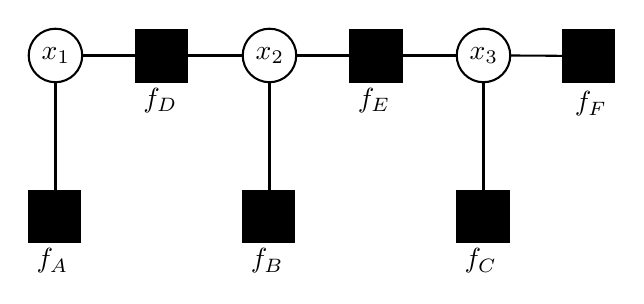
\begin{tikzpicture}[x=0.75pt,y=0.75pt,yscale=-1,xscale=1]
%uncomment if require: \path (0,288); %set diagram left start at 0, and has height of 288

%Shape: Square [id:dp542094098374186] 
\draw  [fill={rgb, 255:red, 0; green, 0; blue, 0 }  ,fill opacity=1 ] (86.34,228.71) -- (110.92,228.71) -- (110.92,253.29) -- (86.34,253.29) -- cycle ;
%Shape: Rectangle [id:dp9431678202688636] 
\draw  [fill={rgb, 255:red, 0; green, 0; blue, 0 }  ,fill opacity=1 ] (189.45,228.71) -- (214.03,228.71) -- (214.03,253.29) -- (189.45,253.29) -- cycle ;
%Shape: Rectangle [id:dp5515594438313509] 
\draw  [fill={rgb, 255:red, 0; green, 0; blue, 0 }  ,fill opacity=1 ] (292.57,228.71) -- (317.14,228.71) -- (317.14,253.29) -- (292.57,253.29) -- cycle ;
%Shape: Rectangle [id:dp19402149967725735] 
\draw  [fill={rgb, 255:red, 0; green, 0; blue, 0 }  ,fill opacity=1 ] (137.9,151.38) -- (162.47,151.38) -- (162.47,175.96) -- (137.9,175.96) -- cycle ;
%Shape: Rectangle [id:dp9723919948872586] 
\draw  [fill={rgb, 255:red, 0; green, 0; blue, 0 }  ,fill opacity=1 ] (241.01,151.38) -- (265.59,151.38) -- (265.59,175.96) -- (241.01,175.96) -- cycle ;
%Shape: Circle [id:dp9001944284946917] 
\draw   (86,163.41) .. controls (86,156.29) and (91.77,150.52) .. (98.89,150.52) .. controls (106.01,150.52) and (111.78,156.29) .. (111.78,163.41) .. controls (111.78,170.53) and (106.01,176.3) .. (98.89,176.3) .. controls (91.77,176.3) and (86,170.53) .. (86,163.41) -- cycle ;
%Shape: Ellipse [id:dp029985916423680425] 
\draw   (189.11,163.41) .. controls (189.11,156.29) and (194.88,150.52) .. (202,150.52) .. controls (209.12,150.52) and (214.89,156.29) .. (214.89,163.41) .. controls (214.89,170.53) and (209.12,176.3) .. (202,176.3) .. controls (194.88,176.3) and (189.11,170.53) .. (189.11,163.41) -- cycle ;
%Shape: Ellipse [id:dp8505763078012687] 
\draw   (292.22,163.41) .. controls (292.22,156.29) and (297.99,150.52) .. (305.11,150.52) .. controls (312.23,150.52) and (318,156.29) .. (318,163.41) .. controls (318,170.53) and (312.23,176.3) .. (305.11,176.3) .. controls (297.99,176.3) and (292.22,170.53) .. (292.22,163.41) -- cycle ;
%Straight Lines [id:da5591298719832298] 
\draw    (202,176.3) -- (202,236.1) ;
%Straight Lines [id:da8657801799701208] 
\draw    (305.11,176.3) -- (305.11,236.1) ;
%Straight Lines [id:da7323179142438296] 
\draw    (98.89,176.3) -- (98.89,236.1) ;
%Straight Lines [id:da2650402956705291] 
\draw    (141.85,163.41) -- (111.78,163.41) ;
%Straight Lines [id:da6929917679064295] 
\draw    (189.11,163.41) -- (159.04,163.41) ;
%Straight Lines [id:da7044874759875848] 
\draw    (244.96,163.41) -- (214.89,163.41) ;
%Straight Lines [id:da30371490539779855] 
\draw    (292.22,163.41) -- (262.15,163.41) ;
%Shape: Rectangle [id:dp26239558807935515] 
\draw  [fill={rgb, 255:red, 0; green, 0; blue, 0 }  ,fill opacity=1 ] (343.59,151.38) -- (368.16,151.38) -- (368.16,175.96) -- (343.59,175.96) -- cycle ;
%Straight Lines [id:da46629291479421253] 
\draw    (355.87,163.67) -- (318,163.41) ;


% Text Node
\draw (90.75,157.95) node [anchor=north west][inner sep=0.75pt]    {$x_{1}$};
% Text Node
\draw (193.86,157.95) node [anchor=north west][inner sep=0.75pt]    {$x_{2}$};
% Text Node
\draw (296.97,157.95) node [anchor=north west][inner sep=0.75pt]    {$x_{3}$};
% Text Node
\draw (88.3,255) node [anchor=north west][inner sep=0.75pt]    {$f_{A}$};
% Text Node
\draw (191.48,255) node [anchor=north west][inner sep=0.75pt]    {$f_{B}$};
% Text Node
\draw (294.53,255) node [anchor=north west][inner sep=0.75pt]    {$f_{C}$};
% Text Node
\draw (243.04,177.67) node [anchor=north west][inner sep=0.75pt]    {$f_{E}$};
% Text Node
\draw (139.79,177.67) node [anchor=north west][inner sep=0.75pt]    {$f_{D}$};
% Text Node
\draw (347.59,179.36) node [anchor=north west][inner sep=0.75pt]    {$f_{F}$};


\end{tikzpicture}


    \caption[short]{An example of a factor graph}
\end{figure}

The above factor graph represents the following factorisation:

\begin{equation}
    p(X_1, X_2, X_3) = f_A(X_1)f_B(X_2)f_C(X_3)f_D(X_1, X_2)f_E(X_2, X_3)f_F(X_3)
    \label{eqn:factors}
\end{equation}

Suppose we wanted to find the probability that $X_1 = z$ for some value of $z$ using the above factor graph. Then we would need to find:

\begin{equation}
    p(X_1 = z, X_2, X_3) = \underset{i=X_2}{\sum} \underset{j=X_3}{\sum} p(X_1 = z, X_2 = i, X_3 =j)
    \label{eqn:bp_derivation_1}
\end{equation}

And by \ref{eqn:factors} we get:

\begin{equation}
    p(X_1 = z, X_2, X_3) = \underset{i=X_2}{\sum} \underset{j=X_3}{\sum} f_A(z)f_B(i)f_C(j)f_D(z, i)f_E(z, j)f_F(j)
\end{equation}


which can be rearranged to form:

\begin{equation}
    p(X_1 = z, X_2, X_3) = f_A(z) \underset{i=X_2}{\sum} \left(f_D(z, i)f_B(i) \left(\underset{j=X_3}{\sum} f_E(z, j)f_C(j)f_F(j) \right)\right)
    \label{eqn:x1}
\end{equation}

Similarly, if we wanted to find the probability that $X_2 = z$ for some z we would need to find:

\begin{equation}
    p(X_1, X_2 = z, X_3) = f_b(z) \left(\underset{i=X_1}{\sum} f_D(i, z) f_A(i)\right) \left(\underset{j=X_3}{\sum} f_E(z, j) f_C(j) f_F(j)\right)
    \label{eqn:x2}
\end{equation}

Noticing how the sum over $X_3$ in both \ref{eqn:x1} and \ref{eqn:x2} is the same, we may want to ``cache'' the result when dealing with large factor graphs, to improve performance. To do this we can associate calculations with nodes in the factor graph. We call these associations ``messages''.

The general form of a message from variable $i$ to factor $j$ is the product of the messages from all other neighbouring factors \cite{GaussianBP}. Put formally:

\begin{equation}
    m_{x_i \rightarrow f_j} = \underset{s \in N(i) \backslash j }{\prod} m_{f_s \rightarrow x_i}
    \label{eqn:v_f}
\end{equation}

The general form of a message from factor $j$ to variable $i$ is the product of the messages from all other neighbouring variables and the factor applied to all other variables except $i$ \cite{GaussianBP}. Put formally:

\begin{equation}
    m_{f_j \rightarrow x_i} = \left(\underset{X_j \backslash x_i}{\sum} f_j(X_j)\right) \left(\underset{k \in N(j) \backslash i}{\prod} m_{x_k \rightarrow f_j}\right)
    \label{eqn:f_v}
\end{equation}

Finally, the marginal value of a variable is simply the product of all incoming messages to it \cite{GaussianBP}.

\begin{equation}
    p(x_i) = \underset{s \in N(i)}{\prod} m_{f_s \rightarrow x_i}
    \label{eqn:bp_belief}
\end{equation}

\subsection{Belief Propagation}
The above equations are used by the Belief Propagation algorithm, an iterative algorithm used to calculate the marginal value for each variable in a factor graph \cite{GaussianBP}. Each iteration of Belief Propagation has 3 phases:

\begin{enumerate}
    \item Variables send messages to each of their neighbouring factors \ref{eqn:v_f}.
    \item Factors send messages to each of their neighbouring variables \ref{eqn:f_v}.
    \item Each variable updates its ``belief'' (its estimated marginal value) \ref{eqn:bp_belief}.
\end{enumerate}

The original Belief Propagation algorithm was designed to be used in tree-like graphs, i.e. graphs without loops \cite{GaussianBP}. However, empirical evidence has shown that ``Loopy-BP'' can still converge to provide useful results in a variety of problem domains \cite{GaussianBP}. % TODO replace citations with better ones 

\subsection{Gaussian Belief Propagation}
Gaussian Belief Propagation is a special case of the Belief Propagation algorithm where the underlying distribution of each variable follows a Gaussian distribution \cite{GaussianBPOriginal}.

% needs a linear relationship between the factors and the variables
\subsection{Lie Theory}
% Lie theory is a thing that can be used to represent positions and stuff
% Fun fact you can use it to apply Gaussians to movement, which is what we do in robot web

\subsection{Putting it all together}

\section{Security Issues}
\subsection{Byzantine fault tolerance}
\subsection{Masquerade Attacks}
\subsection{Sybil Attacks}

